\documentclass[UTF8]{article}
\usepackage{graphicx}
\usepackage{subfigure}
\usepackage{amsmath}
\usepackage{makecell}
\usepackage[utf8]{inputenc}
\usepackage[space]{ctex} %中文包
\usepackage{listings} %放代码
\usepackage{xcolor} %代码着色宏包
\usepackage{CJK} %显示中文宏包
\usepackage{float}
\usepackage{diagbox}
\usepackage{bm}
\usepackage{ulem} 
\usepackage{amssymb}
\usepackage{soul}
\usepackage{color}
\usepackage{geometry}
\usepackage{fancybox} %花里胡哨的盒子
\usepackage{xhfill} %填充包, 可画分割线 https://www.latexstudio.net/archives/8245
\usepackage{multicol} %多栏包
\usepackage{enumerate} %可以方便地自定义枚举标题
\usepackage{multirow} %表格中多行单元格合并
\usepackage{wasysym} %可以使用wasysym里的一堆奇奇怪怪的符号
\usepackage{hyperref} % url
%%%%%%%%%%%%%%%伪代码%%%%%%%%%%%%%%%
\usepackage{amsmath}
\usepackage{algorithm}
\usepackage{algorithmicx}
\usepackage[noend]{algpseudocode}
%%%%%%%%%%%%%%%画图包%%%%%%%%%%%%%%%
\usepackage{tikz}
\usepackage{pgfplots} % http://pgfplots.sourceforge.net/gallery.html
\usetikzlibrary{pgfplots.patchplots} % 拟合支持
\usetikzlibrary{arrows,shapes,automata,petri,positioning,calc} % 状态图支持
\usetikzlibrary{arrows.meta} % 箭头
\usetikzlibrary{shadows} % 阴影支持
\usepackage{forest} % 画树

\geometry{left = 1.5cm, right = 1.5cm, top=1.5cm, bottom=2cm}

\definecolor{mygreen}{rgb}{0,0.6,0}
\definecolor{mygray}{rgb}{0.5,0.5,0.5}
\definecolor{mymauve}{rgb}{0.58,0,0.82}
\lstset{
	backgroundcolor=\color{white}, 
	%\tiny < \scriptsize < \footnotesize < \small < \normalsize < \large < \Large < \LARGE < \huge < \Huge
	basicstyle = \footnotesize,       
	breakatwhitespace = false,        
	breaklines = true,                 
	captionpos = b,                    
	commentstyle = \color{mygreen}\bfseries,
	extendedchars = false,
	frame = shadowbox, 
	framerule=0.5pt,
	keepspaces=true,
	keywordstyle=\color{blue}\bfseries, % keyword style
	language = C++,                     % the language of code
	otherkeywords={string}, 
	numbers=left, 
	numbersep=5pt,
	numberstyle=\tiny\color{mygray},
	rulecolor=\color{black},         
	showspaces=false,  
	showstringspaces=false, 
	showtabs=false,    
	stepnumber=1,         
	stringstyle=\color{mymauve},        % string literal style
	tabsize=4,          
	title=\lstname           
}

%\sum\nolimits_{j=1}^{M}   上下标位于求和符号的水平右端,
%\sum\limits_{j=1}^{M}   上下标位于求和符号的上下处,
%\sum_{j=1}^{M}  对上下标位置没有设定,会随公式所处环境自动调整。

%%%%%%%%%%%%%画图包%%%%%%%%%%%%%
\usepackage{tikz}
%%%%%%%%%%%%%好看的矩形%%%%%%%%%%%%%
\tikzset{
  rect1/.style = {
    shape = rectangle,% 指定样式
    minimum height=2cm,% 最小高度
    minimum width=4cm,% 最小宽度
    align = center,% 文字居中
    drop shadow,% 阴影
  }
}
%%%%%%%%%%%%%画图背景包%%%%%%%%%%%%%
\usetikzlibrary{backgrounds}

%%%%%%%%%%%%%在tikz中画一个顶点%%%%%%%%%%%%%
%%%%%%%%%%%%%#1:node名称%%%%%%%%%%%%%
%%%%%%%%%%%%%#2:位置%%%%%%%%%%%%%
%%%%%%%%%%%%%#3:标签%%%%%%%%%%%%%
\newcommand{\newVertex}[3]{\node[circle, draw=black, line width=1pt, scale=0.8] (#1) at #2{#3}}
%%%%%%%%%%%%%在tikz中画一条边%%%%%%%%%%%%%
\newcommand{\newEdge}[2]{\draw [black,very thick](#1)--(#2)}
%%%%%%%%%%%%%在tikz中放一个标签%%%%%%%%%%%%%
%%%%%%%%%%%%%#1:名称%%%%%%%%%%%%%
%%%%%%%%%%%%%#2:位置%%%%%%%%%%%%%
%%%%%%%%%%%%%#3:标签内容%%%%%%%%%%%%%
\newcommand{\newLabel}[3]{\node[line width=1pt] (#1) at #2{#3}}

%%%%%%%%%%%%%强制跳过一行%%%%%%%%%%%%%
\newcommand{\jumpLine} {\hspace*{\fill} \par}
%%%%%%%%%%%%%关键点指令,可用itemise替代%%%%%%%%%%%%%
\newcommand{\keypoint}[2]{$\bullet$\textbf{#1}\quad#2\par}
%%%%%%%%%%%%%<T>平均值表示%%%%%%%%%%%%%
\newcommand{\average}[1]{\left\langle #1\right\rangle }
%%%%%%%%%%%%%表格内嵌套表格%%%%%%%%%%%%%
\newcommand{\tabincell}[2]{\begin{tabular}{@{}#1@{}}#2\end{tabular}}
%%%%%%%%%%%%%大黑点item头%%%%%%%%%%%%%
\newcommand{\itemblt}{\item[$\bullet$]}
%%%%%%%%%%%%%大圈item头%%%%%%%%%%%%%
\newcommand{\itemc}{\item[$\circ$]}
%%%%%%%%%%%%%大星星item头%%%%%%%%%%%%%
\newcommand{\itembs}{\item[$\bigstar$]}
%%%%%%%%%%%%%右▷item头%%%%%%%%%%%%%
\newcommand{\itemrhd}{\item[$\rhd$]}
%%%%%%%%%%%%%定义为%%%%%%%%%%%%%
\newcommand{\defas}{=_{df}}
%%%%%%%%%%%%%偏导%%%%%%%%%%%%%
\newcommand{\partialx}[2]{\frac{\partial #1}{\partial #2}}
%%%%%%%%%%%%%蕴含%%%%%%%%%%%%%
\newcommand{\imp}{\rightarrow}
%%%%%%%%%%%%%上取整%%%%%%%%%%%%%
\newcommand{\ceil}[1]{\lceil#1\rceil}
%%%%%%%%%%%%%下取整%%%%%%%%%%%%%
\newcommand{\floor}[1]{\lfloor#1\rfloor}

%%%%%%%%%%%%%双线分割线%%%%%%%%%%%%%
\newcommand*{\doublerule}{\hrule width \hsize height 1pt \kern 0.5mm \hrule width \hsize height 2pt}
%%%%%%%%%%%%%双线中间可加东西的分割线%%%%%%%%%%%%%
\newcommand\doublerulefill{\leavevmode\leaders\vbox{\hrule width .1pt\kern1pt\hrule}\hfill\kern0pt }
%%%%%%%%%%%%%左大括号%%%%%%%%%%%%%
\newcommand{\leftbig}[1]{\left\{\begin{array}{l}#1\end{array}\right.}
%%%%%%%%%%%%%矩阵%%%%%%%%%%%%%
\newcommand{\mat}[2]{\left[\begin{array}{#1}#2\end{array}\right]}
%%%%%%%%%%%%%可换行圆角文本框%%%%%%%%%%%%%
\newcommand{\ovalboxn}[1]{\ovalbox{\tabincell{l}{#1}}}
%%%%%%%%%%%%%设置section的counter, 使从1开始%%%%%%%%%%%%%
\setcounter{section}{0}

%%%%%%%%%%%%%Colors%%%%%%%%%%%%%
\newcommand{\lightercolor}[3]{% Reference Color, Percentage, New Color Name
    \colorlet{#3}{#1!#2!white}
}
\newcommand{\darkercolor}[3]{% Reference Color, Percentage, New Color Name
    \colorlet{#3}{#1!#2!black}
}
\definecolor{aquamarine}{rgb}{0.5, 1.0, 0.83}
\definecolor{Seashell}{RGB}{255, 245, 238} %背景色浅一点的
\definecolor{Firebrick4}{RGB}{255, 0, 0}%文字颜色红一点的
\lightercolor{gray}{20}{lgray}
\newcommand{\hlg}[1]{
	\begingroup
		\sethlcolor{lgray}%背景色
		\textcolor{black}{\hl{\mbox{#1}}}%textcolor里面对应文字颜色
	\endgroup
}


\title{机器学习概论 实验报告 \\ \Large Lab3: XGBoost}

\begin{document}
\maketitle
\tableofcontents
\newpage
\section{算法数学基础}
\noindent \hlg{\textbf{XGBoost}}: e\textbf{X}treme \textbf{G}radient \textbf{Boost}ing, 最初是由 陈天奇 负责的研究项目, 后来其在各种数据挖掘比赛表现出了极大的性能优势.
\subsection{提升树}
\subsubsection{基本思想}
\noindent 如果一个预测问题中, 训练的模型(称为 Model1)效果不好, 误差比较大, 我们可以通过基于残差的训练来拟合 Model2, 甚至 Model3, Model4,...
\begin{figure}[H]
	\centering
	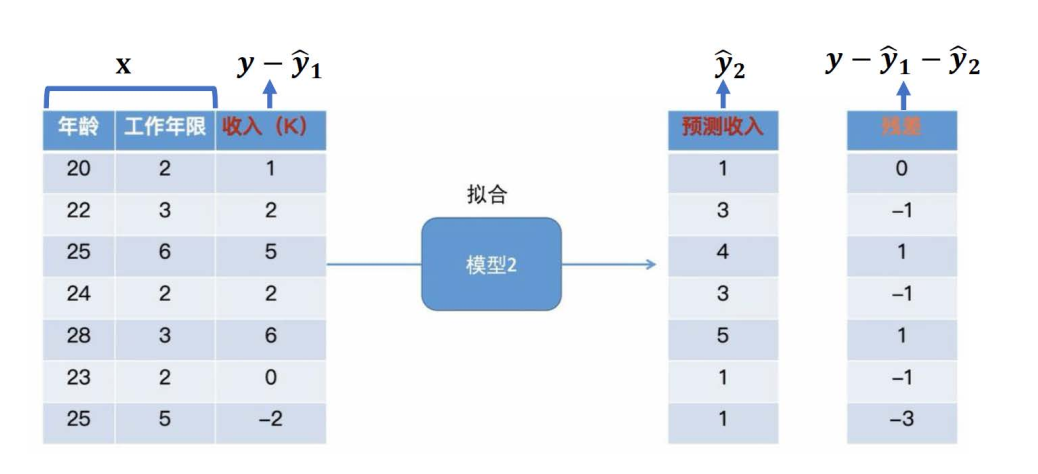
\includegraphics[width=\linewidth*5/8]{model2.png}
	\caption{基于 Model1 的残差训练 Model2}
\end{figure}\par
\noindent于是, 最后将各个模型的结果相加即可得到一个更优的模型. 这就是其基本思想.
\begin{figure}[H]
	\centering
	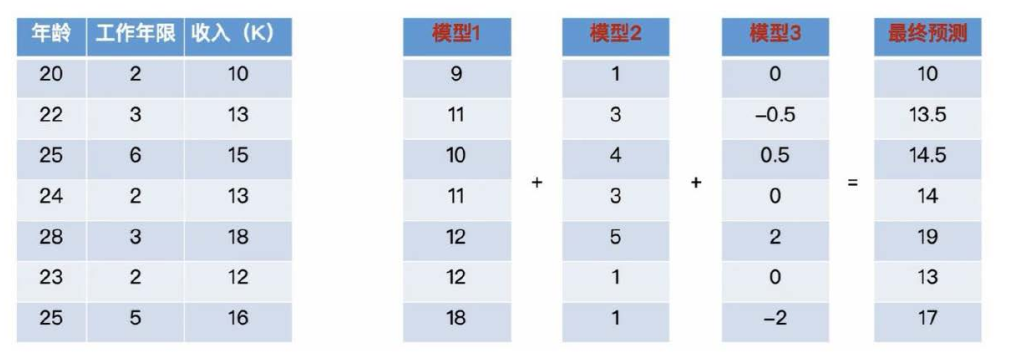
\includegraphics[width=\linewidth*5/8]{model1234.png}
	\caption{最后叠加每个模型的结果}
\end{figure}\par
\subsubsection{相关公式}
\noindent 现在不妨考虑已经训练了 $K$ 棵树, 则对第 $i$ 个样本的预测为:
$$\hat{y}_i=\phi(x_i)=\sum\limits_{i=1}^Kf_k(x_i), f_k\in\mathcal{F}$$
这里目标函数为
$$\mathcal{L}(\phi)=\sum\limits_{i}l(\hat{y}_i,y_i)+\sum\limits_k\Omega(f_k)$$
其中第一项为 训练误差, 第二项为正则化项(可以是叶节点个数, 叶节点评分, 树的深度等)
\subsection{Gradient Tree Boost}
\subsubsection{目标函数与最优权重}
\noindent 考虑第 $i$ 轮的预测为:
$$\hat{y}_i^{(t)}=\hat{y}_i^{(t-1)}+f_t(x_i),$$
那么我们的目标函数就是
$$Obj^{(t)}=\left(\sum\limits_{i=1}^nl(y_i,\hat{y}_i^{(t-1)}+f_t(x_i))\right)+\Omega(f_t)+constant$$
我们可以对目标函数中的训练误差项目, 进行泰勒展开, 并忽略常数项:
\begin{align*}
    \tilde{L}^{(t)}&=\sum\limits_{i=1}^n [g_if_t(\textbf{x}_i) + \frac{1}{2}h_if_t(\textbf{x}_i)]+\Omega(f_t)\\
    &=\sum\limits_{i=1}^n [g_if_t(\textbf{x}_i) + \frac{1}{2}h_if_t(\textbf{x}_i)]+\gamma T+\frac{1}{2}\lambda\sum\limits_{j=1}^T\omega_j^2\\
    &=\sum\limits_{j=1}^T\left[\left(\sum\limits_{i\in I_j}g_i\right)\omega_j+\frac{1}{2}\left(\sum\limits_{i\in I_j}h_i +\lambda \right)\omega^2_j\right]+\gamma T
\end{align*}
这里有$g_i=\partial_{\hat{y}^{(t-1)}}l(y_i,\hat{y}_i^{(t-1)})$ 及$h_i=\partial^2_{\hat{y}^{(t-1)}}l(y_i,\hat{y}_i^{(t-1)})$\\
因此, 进一步我们能得到, 对于一个固定的树结构, 最优的叶子权重为:
$$\omega^*_j=-\frac{\sum_{i\in I_j}g_i}{\sum_{i\in I_j}h_i+\lambda},$$
而相应的最优值则为
$$\tilde{\mathcal{L}}^{(t)}(q)=-\frac{1}{2}\sum\limits_{j=1}^T\frac{\left(\sum_{i\in I_j}g_i\right)^2}{\sum_{i\in I_j}h_i+\lambda}+\gamma T.$$
\subsubsection{split 的准则}
根据上节给出的 $\tilde{\mathcal{L}}$, 我们很容易得到, 将叶子 split 的收益:
$$\mathcal{L}_{split}=\frac{1}{2}\left[\frac{\left(\sum_{i\in I_L}g_i\right)^2}{\sum_{i\in I_L}h_i+\lambda}+\frac{\left(\sum_{i\in I_R}g_i\right)^2}{\sum_{i\in I_R}h_i+\lambda}-\frac{\left(\sum_{i\in I}g_i\right)^2}{\sum_{i\in I}h_i+\lambda}\right]$$

\section{算法过程简介}
\noindent 根据上面的 split 准则, 我们可以设计这样的算法来计算最优 split 方法. 注意其中采用了按每个属性, 从小到大逐个分开地枚举, 从而贪心地得到当前最优 split 方法.
\begin{algorithm}[H]
	\caption{{\sc Pisano-Delete}(H,x)}
	\begin{algorithmic}[1] %每行显示行号
		\Require I, instance set of current node
		\Require m, feature dimension
		\State $gain \leftarrow 0$
		\State $G \leftarrow \sum_{i\in I}g_i, H \leftarrow \sum_{i\in I}h_i $
		\For{$k=1$ to $m$}
			\State $G_L\leftarrow 0, H_L\leftarrow 0$
			\For{$j$ in $sorted(I, by\ x_{jk})$}
				\State $G_L\leftarrow G_L+g_j,\ H_L\leftarrow H_L+h_j$
				\State $G_R\leftarrow G-G_L,\ H_R\leftarrow H-H_L$
				\State $score \leftarrow \max\left(score, \frac{G_L^2}{H_L+\lambda}+\frac{G_R^2}{H_R+\lambda}-\frac{G^2}{H+\lambda}\right)$
			\EndFor
		\EndFor
		\State \Return split with max score
	\end{algorithmic}
\end{algorithm}



\end{document}





